\documentclass[lettersize,journal,12pt]{IEEEtran}
\usepackage{fontspec}
\usepackage{amsmath,amsfonts}
\usepackage{algorithmic}
\usepackage{algorithm}
\usepackage{array}
\usepackage[caption=false,font=normalsize,labelfont=sf,textfont=sf]{subfig}
\usepackage{textcomp}
\usepackage{stfloats}
\usepackage{url}
\usepackage{verbatim}
\usepackage{xeCJK}
\usepackage{lettrine}
\usepackage{graphicx}
\usepackage{titling}
\usepackage{titlesec}
\usepackage{balance}
\usepackage{textcase}
\usepackage{setspace}
\setmainfont{Times New Roman}[SmallCapsFont=TeX Gyre Termes:+smcp]
% rule to break words
\hyphenation{}
\def\BibTeX{{\rm B\kern-.05em{\sc i\kern-.025em b}\kern-.08em
T\kern-.1667em\lower.7ex\hbox{E}\kern-.125emX}}
\pretitle{\begin{center}\fontsize{16}{18}\selectfont\bfseries}
\posttitle{\end{center}}
\preauthor{\begin{center}\fontsize{10}{12}\selectfont}
\postauthor{\end{center}}
\predate{\begin{center}\fontsize{10}{12}\selectfont}
\postdate{\end{center}}
\titleformat{\section}
{\filcenter\fontsize{14}{16}\bfseries\uppercase}
{\thesection}
{1em}
{}
\renewenvironment{abstract}
{\fontsize{12}{14}\textit{\textbf{\abstractname---}}\bfseries\ignorespaces}
{}
\renewenvironment{IEEEkeywords}
{\fontsize{12}{14}\textit{\textbf{Keywords---}}\bfseries\ignorespaces}{}
\begin{document}
\onehalfspacing
\title{Unveiling the PageRank Algorithm: Principles, Performance, and Enhancements}
\author{Wu Zelin, Wu Zekai, Li Pengda
	\thanks{We should thank Miss.Ye here}}

\maketitle\thispagestyle{headings}
\markboth{10225101428 吴泽霖\quad10225101429 武泽恺\quad10225101460 李鹏达}{}%

\begin{abstract}
	This is the abstract area. We should write a very nb abstract here.
\end{abstract}

\begin{IEEEkeywords}
	Keyword1, Keyword2, Keyword3
\end{IEEEkeywords}


\section{Introduction}
\lettrine{T}{his}
is the Introduction area. We should write a very nb introduction here.

\section{The 2nd Section}

This is a simple section.
\subsection{The 2nd Section 1st Subsection}

This is a simple subsection.
This is a simple subsection.
This is a simple subsection.
This is a simple subsection.
This is a simple subsection.
This is a simple subsection.
This is a simple subsection.
This is a simple subsection.
This is a simple subsection.
This is a simple subsection.
This is a simple subsection.
This is a simple subsection.
This is a simple subsection.
This is a simple subsection.
This is a simple subsection.
This is a simple subsection.
This is a simple subsection.
This is a simple subsection.
This is a simple subsection.
This is a simple subsection.
This is a simple subsection.
This is a simple subsection.
This is a simple subsection.
This is a simple subsection.
This is a simple subsection.
This is a simple subsection.
This is a simple subsection.
This is a simple subsection.
This is a simple subsection.
This is a simple subsection.

\subsection{The 2nd Section 2nd Subsection}

This is a simple subsection too.
\section{The 3rd Section}

This is a simple section.
\subsection{The 3rd Section 1st Subsection}

This is a simple subsection. We can make a citation here. \cite{ref1}

\figurename~\ref{fig1} is a figure. You can see it at the top of the page.

\begin{figure}[!t]
	\centering
	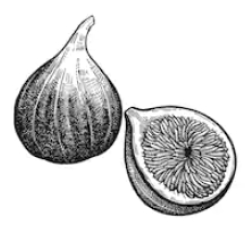
\includegraphics[width=2.5in]{images/fig1.png}
	\caption{This is a figure.}
	\label{fig1}
\end{figure}

\subsection{The 3rd Section 2nd Subsection}

This is a simple subsection too.
\section{The 4th Section}

This is a simple section.
\subsection{The 4th Section 1st Subsection}

This is a simple subsection.

This is an equation:

\begin{equation}
	\label{eq:1}
	e^{\pi i} + 1 = 0
\end{equation}
You can ref it by see\eqref{eq:1}.

\subsection{The 4th Section 2nd Subsection}

This is a simple subsection too.

This is a algorithm:

\begin{algorithm}[H]
	\caption{Weighted Tanimoto ELM.}\label{alg:alg1}
	\begin{algorithmic}
		\STATE
		\STATE {\textsc{TRAIN}}$(\mathbf{X} \mathbf{T})$
		\STATE \hspace{0.5cm}$ \textbf{select randomly } W \subset \mathbf{X}  $
		\STATE \hspace{0.5cm}$ N_\mathbf{t} \gets | \{ i : \mathbf{t}_i = \mathbf{t} \} | $ \textbf{ for } $ \mathbf{t}= -1,+1 $
		\STATE \hspace{0.5cm}$ B_i \gets \sqrt{ \textsc{max}(N_{-1},N_{+1}) / N_{\mathbf{t}_i} } $ \textbf{ for } $ i = 1,...,N $
		\STATE \hspace{0.5cm}$ \hat{\mathbf{H}} \gets  B \cdot (\mathbf{X}^T\textbf{W})/( \mathbb{1}\mathbf{X} + \mathbb{1}\textbf{W} - \mathbf{X}^T\textbf{W} ) $
		\STATE \hspace{0.5cm}$ \beta \gets \left ( I/C + \hat{\mathbf{H}}^T\hat{\mathbf{H}} \right )^{-1}(\hat{\mathbf{H}}^T B\cdot \mathbf{T})  $
		\STATE \hspace{0.5cm}\textbf{return}  $\textbf{W},  \beta $
		\STATE
		\STATE {\textsc{PREDICT}}$(\mathbf{X} )$
		\STATE \hspace{0.5cm}$ \mathbf{H} \gets  (\mathbf{X}^T\textbf{W} )/( \mathbb{1}\mathbf{X}  + \mathbb{1}\textbf{W}- \mathbf{X}^T\textbf{W}  ) $
		\STATE \hspace{0.5cm}\textbf{return}  $\textsc{sign}( \mathbf{H} \beta )$
	\end{algorithmic}
	\label{alg1}
\end{algorithm}

\begin{thebibliography}{1}

	\bibitem{ref1}
	S. Zhan, S. Li and W. Wang, {\it{A Very Nb Book}}. Shanghai, P.R.C., East China Normal  Univ. Press, 2022.

\end{thebibliography}

\end{document}


